\section{Approach} 

There are countless different approaches one could take to calibrate a camera, 

A camera model is a projection model which approximates the function of a camera by describing a mathematical relationship between points in 3D space and its projection onto the sensor grid of the camera. In order to construct such a model, we must first understand the general workings of a camera.

however they all build upon techniques first described in multiple highly influential papers, most notably Tsai's ``A Versatile Camera Calibration Technique for High-Accuracy 3D Machine Vision Metrology Using Off-the-shelf TV Cameras and Lenses'' and Zhang's ``A Flexible New Technique for Camera Calibration''. 

\subsection{Camera Model} \label{sec:camera_model}

The modern lens camera is highly sophisticated, built with an array of complex mechanisms and a wide range of features such as zoom and autofocus. However, we only need to focus on its three principal elements critical to image projection: the lens, the aperture, and the sensor grid (CCD). 

\begin{itemize}[leftmargin=!, itemindent=-5ex]
    \item \textbf{Lens} -- Focuses incoming light rays and projects it onto the sensor grid. Modern cameras have compound lenses (lenses made up of several lens elements) in order to minimize undesired effects such as aberration, blurriness, and distortion. 
    \item \textbf{Aperture} -- Controls the amount of light that reaches the sensor. By adjusting the aperture size, the exposure and depth of field can be modified.
    \item \textbf{Sensor Grid} -- Captures the projected image
\end{itemize}

\begin{figure}[H]
    \centering
    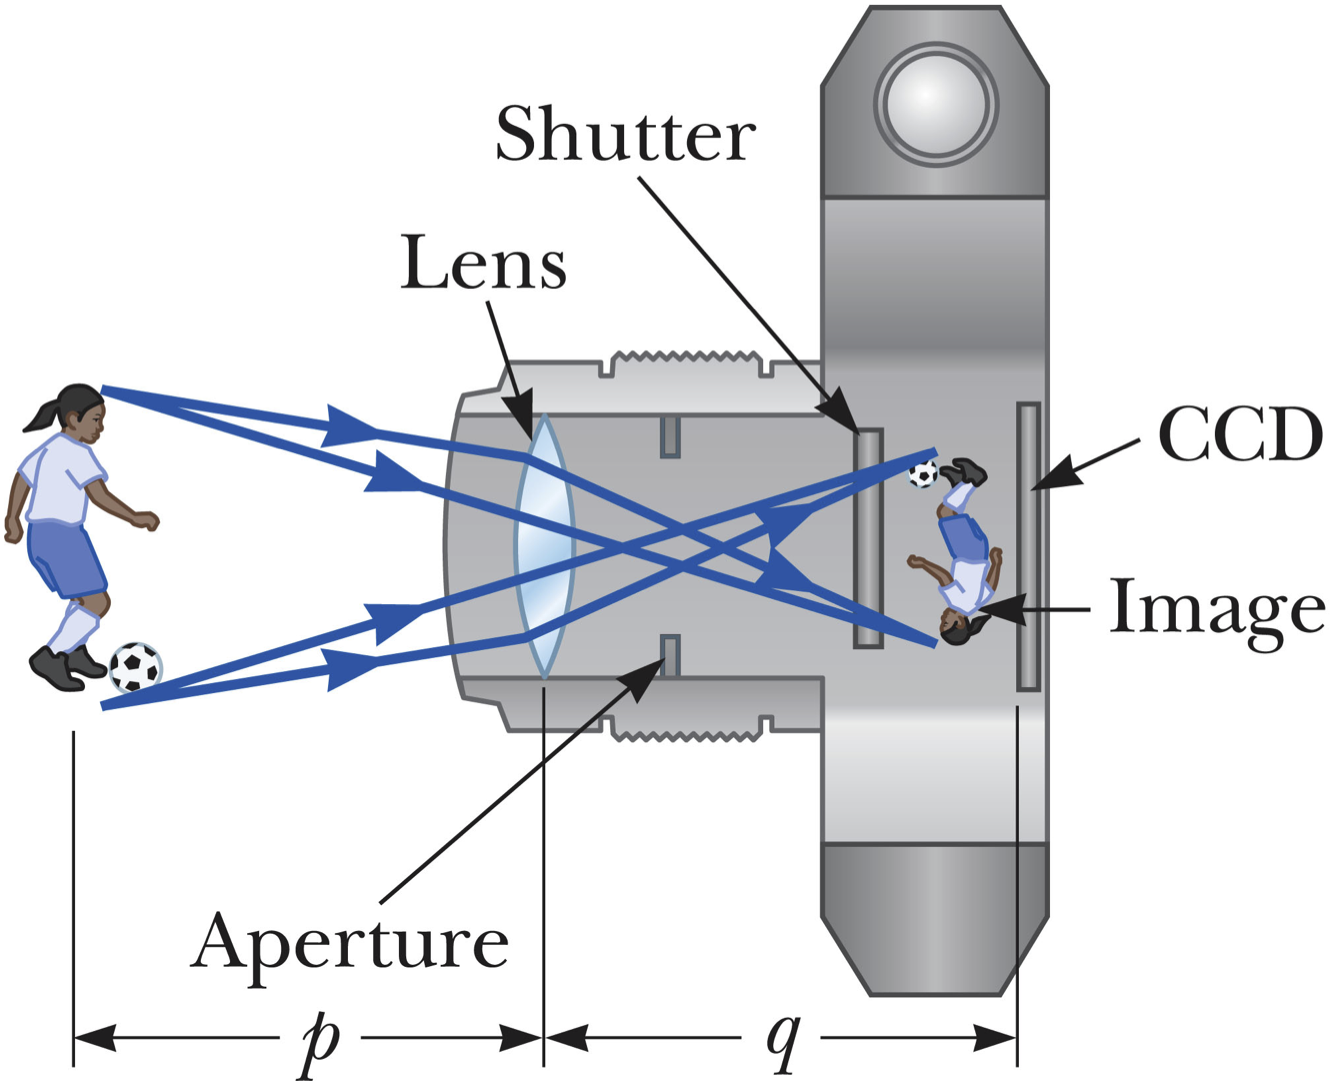
\includegraphics[width=0.5\textwidth]{images/lens_camera}
    \caption{Lens camera. Adapted from \cite{coltonPhysics1232012}} \label{fig:lens_camera}
\end{figure}

However, even this simplified model of a lens camera is still too complicated to describe, as it is impossible to encapsulate the complex behavior of a lens succinctly using one simple mathematical equation. As such, it is mathematically convenient to approximate the camera as a pinhole camera. In doing so, we ignore lens distortion, but it distills the behavior of a camera to its most fundamental and essential dynamics: the projection of points in 3D space onto the flat 2D sensor plane. 

\subsubsection{Pinhole Camera Model}

A pinhole camera is a simple camera without a lens. It instead relies on the use of a tiny hole as the aperture of the camera, and light rays pass through the hole, projecting an inverted image onto the image plane. The pinhole camera model is based on the pinhole camera, however it goes further by making the assumptions that the aperture is infinitely small. This means that any incoming light ray can only travel straight through the pinhole, and that a point in space can only map to one single point on image plane. 

\begin{figure}
    \centering
    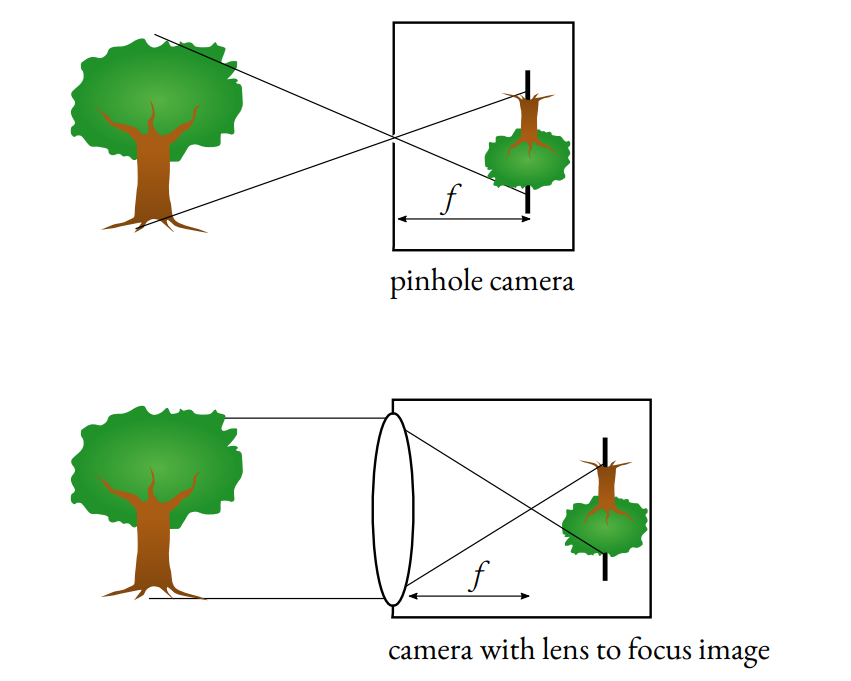
\includegraphics[width=0.7\textwidth]{images/pinhole_vs_lens}
    \caption{Difference between a pinhole camera and a lens camera. Adapted from \cite{leCameraModel2018}}
\end{figure}

If necessary, one could reintroduce distortion and shear terms in order to minimize the error, but this is often not needed for low to medium precision applications, as the distortion of modern lenses are already minimal. As such, its ease of use has led it to become one of the most frequently employed camera models in the field of camera calibration. 

\subsection{Calibration Object}

The calibration object is an object with known dimensions 


Calibration objects can be roughly separated into 3 categories, based on the dimension of the calibration object used \footcite{zhangCameraCalibration2007}:

\begin{itemize}[leftmargin=!, itemindent=-4ex]
    \item \textbf{3D} -- 
    \item \textbf{2D} -- 
    \item \textbf{1D} -- 
\end{itemize}
